\documentclass[11pt,utf8]{article}
\usepackage[utf8]{inputenc}
\usepackage[francais]{babel}
\usepackage{graphicx}
%\usepackage[latin1]{inputenc}
%\usepackage[french]{babel}
\usepackage{amsmath,amssymb,amsfonts}
\usepackage{hyperref}
\hypersetup{
     colorlinks   = true,
     citecolor    = gray
} 
 \usepackage{amsmath,scalerel}
\usepackage{textcomp}
\usepackage{enumerate}% http://ctan.org/pkg/enumerate

\DeclareMathOperator*{\Bigcdot}{\scalerel*{\cdot}{\bigodot}}


\usepackage{colortbl,booktabs}
\usepackage{listings}
\usepackage{pgfplots,pgfplotstable}
\usepackage{xspace}
\usepackage{tikz}
\usetikzlibrary{arrows,patterns,plotmarks,shapes,snakes,er,3d,automata,backgrounds,topaths,trees,petri,mindmap}


\definecolor{lbcolor}{rgb}{0.95,0.95,0.95}
\definecolor{cblue}{rgb}{0.,0.0,0.6}

\newcommand{\Air}{\text{\textsc{Air}}\xspace}
\newcommand{\PCB}{\text{\textsc{PCB}}\xspace}
\newcommand{\IC}{\text{\textsc{IC}}\xspace}
\newcommand{\ICs}{\text{\textsc{ICs}}\xspace}

\newcommand{\OPUS}{\textsc{OPUS}\xspace}
\newcommand{\FF}{\textsc{Freefem++}\xspace}
\newcommand{\COMSOL}{\textsc{Comsol}\xspace}
\newcommand{\COMSOLUJF}{\textsc{Comsol(UJF)}\xspace}
\newcommand{\COMSOLEADS}{\textsc{Comsol(EADS)}\xspace}
\newcommand{\Feelpp}{\textsc{Feel++}\xspace}
\newcommand{\GMSH}{\textsc{Gmsh}\xspace}
\newcommand{\BOOST}{\textsc{Boost}\xspace}

\newcommand{\UJF}{\textsc{UJF}\xspace}
\newcommand{\EADS}{\textsc{EADS}\xspace}

\newcommand{\vect}[1]{\ensuremath{\mathbf{#1}}\xspace}


\definecolor{Lightgray}{rgb}{0.85, 0.85, 0.85}

\usepackage{filecontents,listings}
\lstset{language=c++,showspaces=false,showstringspaces=false,captionpos=t,literate={>>}{\ensuremath{>>}}1,mathescape}
\lstset{basicstyle=\small\bf\ttfamily}
\lstset{lineskip=-2pt}

%\lstset{emph={inline},emphstyle=\color{red}\bfseries}

\definecolor{cgreen}{rgb}{0.,0.6,0.0}

\definecolor{violet}{rgb}{0.5,0,0.5}
\definecolor{vertfonce}{rgb}{0.,0.5,0.}
\definecolor{rouge}{rgb}{0.5,0.,0.}
\definecolor{bleu}{rgb}{0.,0.,1}
\definecolor{orange}{rgb}{1,0.5,0}
\lstset{keywordstyle=\color{red}\bfseries}
\lstset{
emph={form,form1,form2,integrate,on,grad,gradt,dot,id,dx,dy,dz,idt,dxt,dyt,dzt,idv,dxv,dy,dzv,gradv,div,divt,divv,dn,jump,trans,vec,cst,
  project,P,Px,Py,Pz,one,oneX,oneY,oneZ,hFace,N,Nx,Ny,Nz,sin,cos,min,max,abs,pow,chi,exp,LinearForm,BilinearForm,MixedLinearForm,MixedBilinearForm,
  FESpace,MixedFESpace,integrate,project,addCL},emphstyle=\color{bleu},
emph={[2]\_space,\_range,\_expr,\_quad,\_quad1,\_test,\_trial,\_matrix,\_vector,\_solution,\_element,\_rhs,\_rowstart,\_colstart,\_block,
  \_pattern,\_pattern\_block,\_domainSpace,\_imageSpace,\_mesh,\_name,\_partitions,\_worldcomm,\_worldscomm,
  \_type,\_marker1,\_marker2,\_marker3,\_marker4,\_marker5,\_marker6,\_marker7,\_marker8,\_markerAll,\_argc,\_argv,\_desc},emphstyle={[2]\color{violet}\bfseries},
emph={[3]elements,markerName,boundaryfaces,markedfaces,\_Q,solve, newMatrix,newVector,newZeroMatrix,newZeroVector,
  newBlockMatrix,newBlockVector,localize,element,apply,createMesh,localSize,subWorldComm,transpose,setMarker,add,save,
  dirichlet\_vec,neumann\_scal,updateTime,exportResults,updateBdf,init,FluidMechanics}, emphstyle={[3]\color{rouge}\bfseries},
emph={[4]Backend,BlocksVector,BlocksSparseMatrix,BlocksStencilPattern,Blocks,opInterpolation,FunctionSpace,Lagrange,bases,Pch,unitSquare,WorldComm,
  Mesh,Simplex,Node,Rectangle,Quadrangle,Circle,AppliManagement,Environment,feel\_options,exporter},emphstyle={[4]\color{orange}\bfseries},
emph={[5]size\_type,uint16\_type},emphstyle={[5]\color{red}\bfseries},
emph={[6]GeoTool,vf,cl},emphstyle={[6]\color{cyan}\bfseries}
}


\lstset{commentstyle=\ttfamily\color{cgreen}}
\lstset{numberstyle=\tiny}
\lstset{backgroundcolor=\color{lbcolor},rulecolor=}

\lstset{frame=single,framerule=0.5pt}
\lstset{belowskip=\smallskipamount}
\lstset{aboveskip=\smallskipamount}
\lstset{includerangemarker=false,rangeprefix=\/\/\#\ ,% curly left brace plus space
  rangesuffix=\ \#}


%--------dimension
\textwidth 185 true mm
\textheight 220 truemm
\voffset -15 true mm
\hoffset -18 true mm

\def \x  {\textbf x}
\def \n  {\textbf n}
\def \cT {{\cal T}}


% above is the preamble
\title{INTERNSHIP REPORT}
\author{PREPARED BY :\\ Kyoshe Winstone\\University of Strasbourg\\STRASBOURG}

\begin{document}

\begin{center}
\textbf{{\large INTERNSHIP REPORT} }\\ % \\ = new line
\end{center}
\begin{center}
\copyright 2015 by Kyoshe Winstone \\
\end{center}

\begin{center}
MASTER 1 CSMI\\
\end{center}
\begin{center}
June 26, 2015

\end{center}
\begin{center}
 
\includegraphics[width=10cm,height=10cm]{p1}
 \end{center}
 \begin{center}
 
\section*{FEEL++  }
\begin{center}
\textbf{{\large  THE FEELPP-DOXYGEN} }\\ % \\ = new line
   \end{center}
\label{weekly report of the internship}

\end{center}
\newpage

\section{Introduction}
Feel++ is a unified C++ implementation of Galerkin methods (finite and spectral element methods) in 1D, 2D And 3D to solve partial differential equations.\\
For this part of the project, we are interested in generating a Doxygen documentation of the Feelpp project, that is to say, set the mechanisms needed to let the user use  \textbf{\textit{make doxy}} in the command line.
We create a CMakLists.txt to enable Doxygen to generate a documentation with the  command line  \textbf{\textit{make doxy}}.\\
In the main CMakeLists.txt, we activate the whole process by setting \\
 FEELPP\textunderscore ENABLE\textunderscore DOCUMENTATION=ON to enable doxygen to generate the documentation.



\section{doxygen/CMakeLists.txt}
The main Goal here is to set a mechanism which will allow a user to use \textbf{\textit{make doxy}} in the command line to generate a doc documentation when desired.Below is a proposed CMakeLists.txt to be added in the feelpp/doc/doxygen folder to configure a working environment for doxygen.


 \begin{center}
 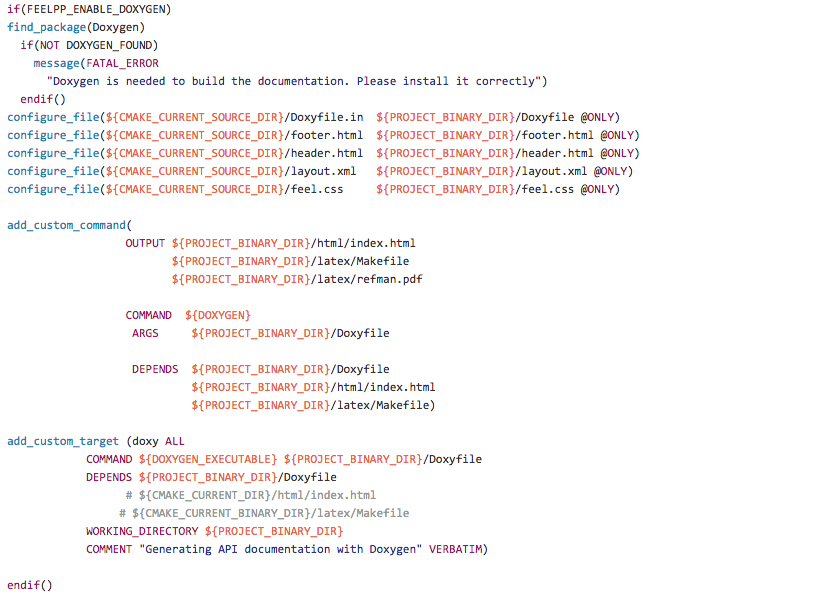
\includegraphics[width=20cm,height=14cm]{im1}
 \end{center}
 
To get this CMakeLists.txt linked to our doc/CMakeLists.tx, we  add a subdirectory(doxy) in the doc/CMakeLists.txt. Now our  doc/CMakeLists.txt, should look like this :

 \begin{center}
 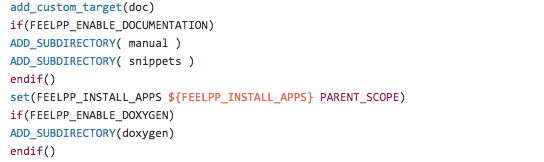
\includegraphics[width=15cm,height=5cm]{im2}
 \end{center}
 

 To generate the Documentation using Doxygen, in the Feelpp directory, we create a temporary \textbf{\textit{build}} directory where all the generated files will be installed. Then we navigate into the  \textbf{\textit{build}} directory and run  \textbf{\textit{cmake ..}} in the command line directing to the feelpp source directory. 
 
 \begin{center}
 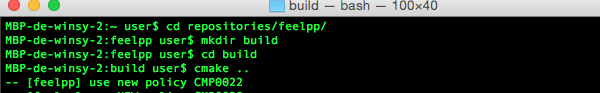
\includegraphics[width=12cm,height=4cm]{img}
 \end{center}
 
 After all the files have been configured, we run "make doxy". At the end of this, we will have the necessary html and latex files to generate the documentation.\\
 \textbf{\textit{NOTE :}}\\
 To reset the  FEELPP\textunderscore ENABLE\textunderscore DOCUMENTATION Option in the command line, use :
 
 \begin{center}
 \begin{lstlisting}
  CMAKE  -DFEELPP_ENABLE_DOCUMENTATION = ON
 \end{lstlisting}
 \end{center}
 
 \section{DIFFICULTIES :}
 \begin{enumerate}[i.]
 \item Using the  \textbf{\textit{open html /index.html}} command in the command line on ATLAS to launch the html online browser of the documentation generated.  That  didn't work for me.\\
\item Using the  \textbf{\textit{pdf latex  ,   pdflatex filename}} command in the command line on ATLAS to get the pdf format of the documentation generated.  That  didn't work either.
 
\end{enumerate}
\newpage
\section{REFERENCES}
\begin{enumerate}[1]
\item \href{http://www.stack.nl/~dimitri/doxygen/manual/docblocks.html.}{DOXYGEN MANUAL}   
\item \href{http://www.cmake.org/cmake/help/v3.0/command/option.html}{CMAKE COMMANDS}
\item \href{http://gl.developpez.com/tutoriel/outil/makefile/}{MAKEFILE TUTORIAL}
 \item \href{http://www.cmake.org/cmake-tutorial/}{CMAKE TUTORIAL}
\end{enumerate}
\end{document}